\chapter{Evaluation}
\label{ch:evaluation}

This chapter evaluates the Basilisk platform based on the developments described in chapter \ref{ch:implementation} and the ease of using the platform to set up a continuous benchmark job for an existing repository.
We will compare the manual benchmarking process using \iguana{} to the use of the Basilisk platform and evaluate the added value the platform creates for the benchmarking process.
\\

The main goal of the platform is to simplify the process of benchmarking known \tsp{}. 
The platform automates the detection of a new release of a configured \ts{} and automates the execution of a benchmark job for the new releases.
%This was not accomplished by any other platform before.
%In our research we did not find a solution that offers the possibility of running automated benchmarks
\\

To evaluate the capabilities of the platform, we set up continuous benchmarks for two different \tsp{}.
The first \ts{} is \tentris{}\footnote{\url{https://tentris.dice-research.org/}}, which is developed by the DICE-research group.
The second \ts{} benchmarked in this thesis is Oxigraph\footnote{\url{https://github.com/oxigraph/oxigraph}}.

The \tsp{} are chosen because they both are available as a ready-to-run docker image on \dockh{}.
They also differ in the way the benchmark dataset is loaded into their internal storage.
The \tentris{} \ts{} accepts the dataset file as an argument at program start, while Oxigraph needs to be started before the data is upoaded through the SPARQL endpoint of the \ts{}.


\section{Initial Benchmark Setup}
In this section, we compare the steps needed for setting up an initial \ts{} benchmark using the \iguana{} framework.
In general, the execution of a benchmark has the following four requirements:
A running \ts{}, the \iguana{} framework, a dataset file, and a query file.

The following two sections describe the initial setup for a manual benchmark run and the recommended process to create a Basilisk configuration for a \ts{}.


\subsection{Manual Benchmark Setup}
\label{sec:eval_manual_benchmark_setup}
To manually run a benchmark, first, the \ts{} needs to be installed and started.
This can be done for a manual test run as a full installation or by using a Docker container.
Often it is easier to use a ready-to-run docker container that contains all needed dependencies and a running installation of the \ts{}.
On the host system, only the Docker engine is needed to run a container.

When the \ts{} is running, the dataset needs to be loaded into the \ts{}.
This can be done either by providing the dataset during startup or by uploading the data through the SPARQL endpoint.
Lastly, the \iguana{} framework needs to be configured by providing a configuration file containing the query file and SPARQL endpoint.

This process is similar for \tentris{} and Oxigraph.
The only difference is in the upload of the dataset.


\subsection{Basilisk Benchmark Setup}
When a \ts{} is fully configured in the Basilisk platform, the platform will automatically provide all four requirements for a benchmark when a new benchmark job is automatically created.
An instance of the \ts{} is started, the \iguana{} framework is configured, and the dataset- and query files are loaded.

To create a working \ts{} configuration for the platform, we recommend developing and testing a local setup first.
The process of creating this initial test setup is similar to the setup of a manual benchmark explained in section \ref{sec:eval_manual_benchmark_setup}.
However in this case, we need to use a Docker container since Basilisk is only working with a container setup.

The local setup should consist of a \ts{} running in a Docker container, which is also reachable over the SPARQL endpoint.
To make sure that \iguana{} is able to perform a benchmark, it is also advised to start a short benchmark with a simple \iguana{} configuration.

The \iguana{} configurations for the tested \tsp{} will slightly differ for loading the dataset into the \ts{}.
In case of \tentris{}, the dataset is configured to be provided inside the Docker container to be loaded on startup.
For Oxigraph, the dataset does not need to be provided inside the Docker container.
In this situation, the dataset needs to be loaded after the startup.
\iguana{} needs to be configured with a pre-hook script that will be executed before the real benchmark starts.
The task of the pre-hook-script is to take a dataset file as input and upload the file to the running Oxigraph instance.
This script should be implemented and tested with the local test setup.

When a working setup is found, the setup can be transferred into the Basilisk platform.
Again, the setup for \tentris{} and Oxigraph are mostly the same.
For Oxigraph, the custom load script is provided, and the Basilisk configuration will point to the script when creating an \iguana{} configuration.



\subsection{Comparison of Initial Setups}
The initial setup to perform one benchmark for one \ts{} version is nearly the same for the manual process as well as for the Basilisk process.
In both scenarios the \ts{} and \iguana{} are setup and run manually.
The configuration of the Basilisk platform is more complicated for the case of loading the dataset through the SPARQL endpoint since a custom load script is needed.
Additionally, the configuration needs to be transferred to the Basilisk platform before a benchmark can be started.


\section{Setup of further Benchmarks}
The real advantage of the Basilisk platform can be seen when further benchmarks have to be run for an already configured \ts{}.

We look into two scenarios that require the run of further benchmarks on a known \ts{}.
Both scenarios will be looked at for the manual setup and an already configured Basilisk setup.
The first scenario is the usage of a different dataset and query file as a new benchmark that is to be run.
The second scenario is the benchmark of a different version of a configured \ts{}.

Both scenarios are evaluated in the following sections.


\subsection{Using a different Benchmark}
In the scenario of using a different benchmark, a new dataset and query file are used.
For the manual setup described in section \ref{sec:eval_manual_benchmark_setup} multiple steps have to be done to update the dataset and query file.
First, the dataset needs to be loaded into the \ts{}.
This can be done by using the SPARQL endpoint to upload the data or by restarting the \ts{} and providing the new dataset at startup.
For \tentris{} it is usually easier to restart the \ts{} with the new dataset as a argument on startup.
Secondly, the \iguana{} configuration needs to be adjusted to use the new query file.
\\

In case of the Basilisk setup, only the new dataset and query file has to be configured in the platform.
When a new benchmark job is executed, the \iguana{} configuration is automatically generated using the new benchmark setup.
If the load-script for Oxigraph is set up correctly, the new dataset will also be automatically uploaded to the \ts{}.
To perform the new benchmark, a manual job can be started by sending a request to the API of the \ac{jms}.


\subsection{Benchmarking a new Triplestore Version}
If a new version of a \ts{} should be benchmarked, again, multiple steps are needed for the manual benchmark process.
The first step is to download the new version and start as a Docker container.
Then, the dataset needs to be loaded into the \ts{}, and lastly, the \iguana{} configuration needs to be updated to the new SPARQL endpoint location.
\\

The Basilisk configuration does not need to be changed.
If a new version has to be benchmarked, either the platform has already noticed the new version on its own and created a new benchmark job automatically, or the user can create a manual benchmark job by providing the benchmark that should be used and the \ts{} version to the API of the \ac{jms}.
The platform will then automatically set up the container and configure \iguana{} to run the benchmark job.
This is the main idea why the platform was originally developed.
Of course, this will only work if the other versions of the \ts{} can use the same basic configuration for the startup, loading the dataset, and providing the SPARQL endpoint.
If there are significant changes to the setup and structure of a \ts{}, a new configuration in Basilisk is needed.


\subsection{Comparison of Benchmark Changes}
As seen in the description of the above scenarios, the \ts{} configuration of the Basilisk platform is not changed at all.
Only the new benchmark files are registered in case a new benchmark should be performed.

In contrast to this, the manual setup requires a lot of manual changes.
Each change to a running configuration requires the user to set up the benchmark configuration from the start.
Either the \ts{} is downloaded and set up again, or the \iguana{} configuration needs manual changes.
This results in a lot of manual work that is often similar to tasks that have been done for other setups.


\section{Basilisk Evaluation}
The idea of the Basilisk platform is focused on the use-case of automatically benchmarking \tsp{} through their SPARQL endpoints.
The Basilisk platform fulfills this task of automating the benchmark process of configured \ts{} repositories stored on \dockh{}.

The comparison of the Basilisk platform to the manual benchmark process shows the advantage of using Basilisk to perform multiple benchmarks on different \ts{} versions.

Setting up the Basilisk platform is initially more complicated and a little more restricted than a manual setup of a \ts{}.
However as soon as the second benchmark is performed, the Basilisk platform has no manual setup time by the user, and the whole process is already faster than a manual approach.
Once the \ts{} is configured, either the benchmark jobs are created automatically by the system, or the user can manually create a job.
The setup and execution of the benchmark job are then done completely automatically by the platform, and no further user interaction is needed.
\\

Using the system, we were able to perform 16 benchmarks on different \tentris{} versions using the \ac{swdf} dataset and query file in just one hour.
It would not be possible to benchmark all versions manually by downloading and setting up the Docker images in a similar time frame.

The \ac{swdf} dataset contains 372K triples with 32K subjects, 96K objects, and 185 predicates.
We were using the same version that was also used in \cite{bigerlTentrisTensorBasedTriple2020}.

Figure \ref{fig:QMPH} shows the number of query mixes that are executed per hour on the different \ts{} versions.
The average of the penalized queries per second is shown in figure \ref{fig:pAvgQPS}.
A query gets penalized if it failed, \eg{} if the timeout is hit, or the \ts{} returned a wrong return code.
Oxigraph seems to have a low QMPH while still having a high average QPS.
We investigated this further in figure \ref{fig:qps} which shows a boxplot of the QPS measurements taken for each query during a benchmark.
For Oxigraph, we can see that some queries have a very low QPS value.
This explains the low QMPH values we see in figure \ref{fig:QMPH}.
The averaged QPS value gets not influenced that much by singular low QPS values, as seen in figure \ref{fig:pAvgQPS}.

All benchmark results are available through the SPARQL endpoint of the Fuseki \ts{} in which the results are written after each benchmark.

\begin{figure}[tbph]
	\centering
	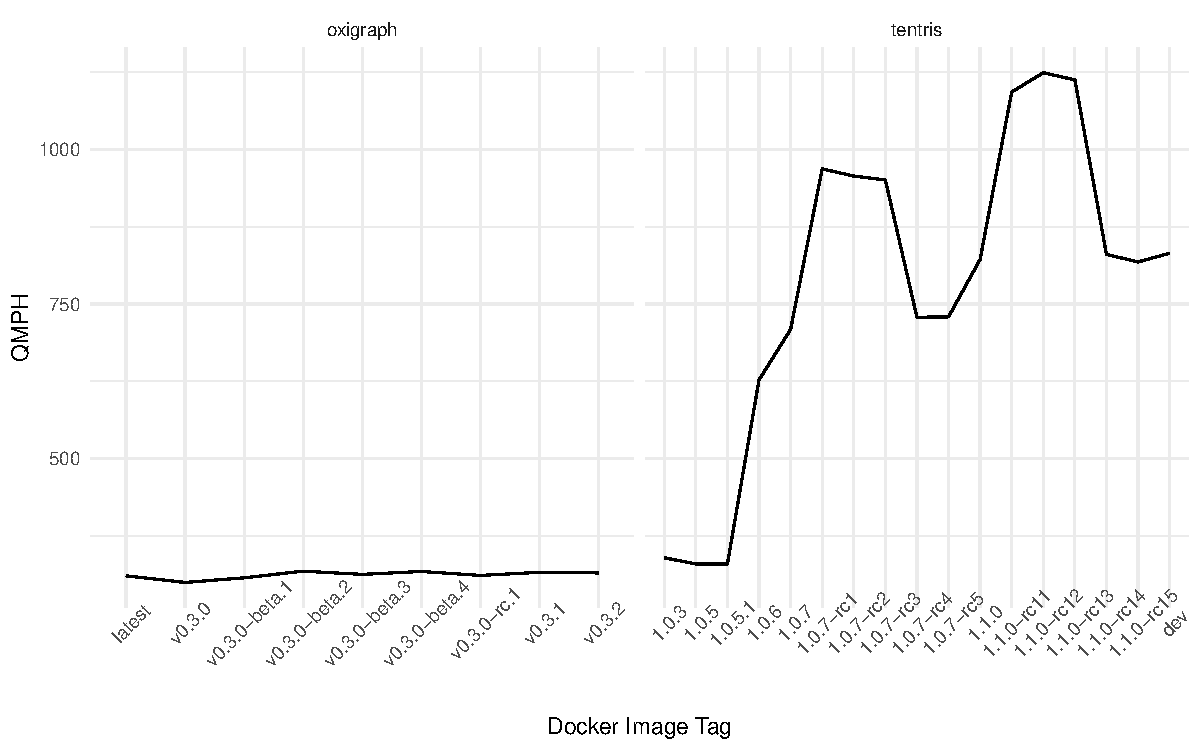
\includegraphics[width=.8\textwidth]{figures/QMPH.pdf}
	\caption{Measured QMPH of the benchmarked \ts{} versions}
	\label{fig:QMPH}
\end{figure}

\begin{figure}[tbph]
	\centering
	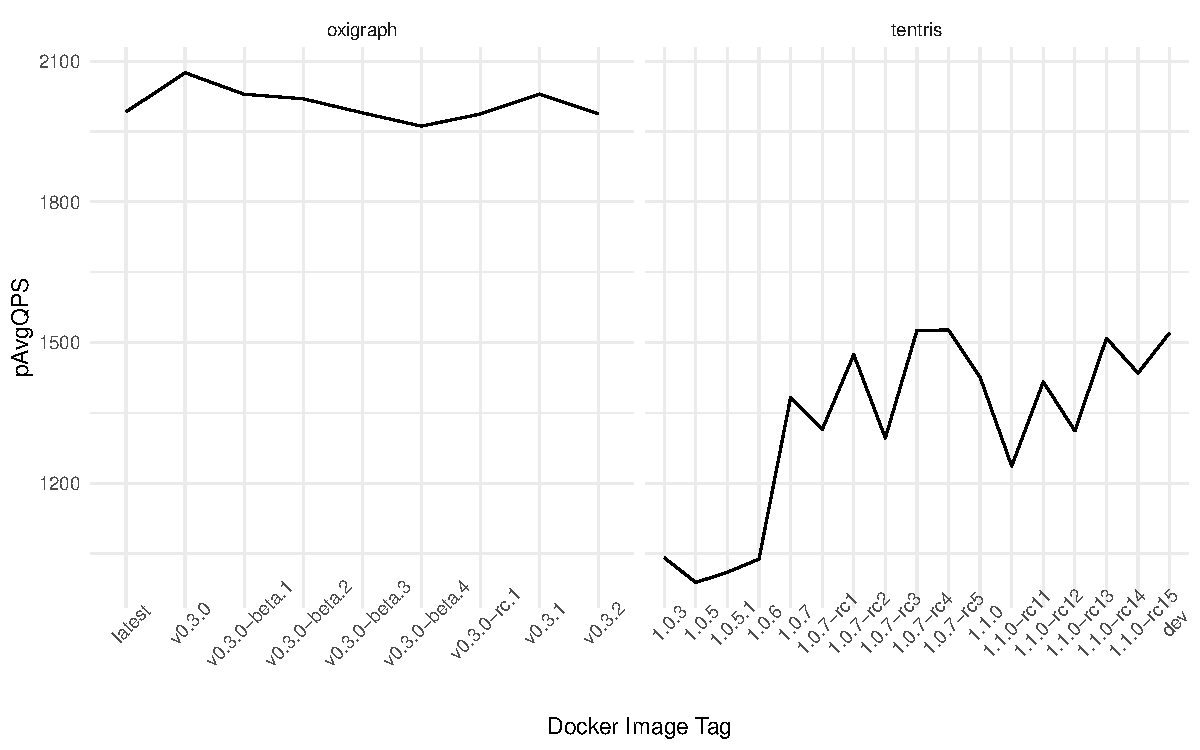
\includegraphics[width=.8\textwidth]{figures/pAvgQPS.pdf}
	\caption{Measured pAvgQPS of the benchmarked \ts{} versions}
	\label{fig:pAvgQPS}
\end{figure}

\begin{figure}[tbph]
	\centering
	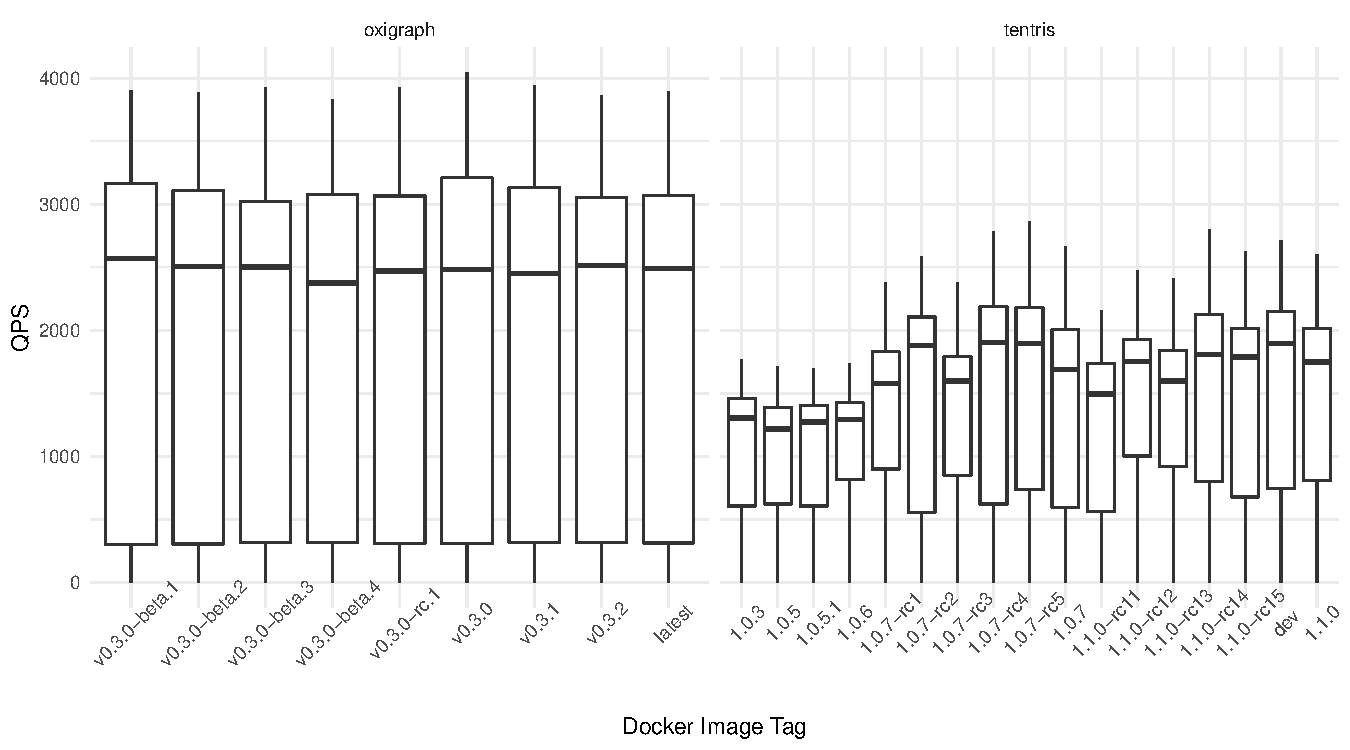
\includegraphics[width=.9\textwidth]{figures/qps.pdf}
	\caption{Boxplot of the QPS of executed queries for each benchmarked \ts{} version}
	\label{fig:qps}
\end{figure}



%This is also the first time the Oxigraph \ts{} is benchmarked independently ??





%%%%%%%%%%%%%%%%%%%%%%%%%
% - Experiment setup, requirements
% - Performing of benchmarks
% - Result evaluation

%- was macht basilisk was vorher nicht da war
%- versch systeme mit selben zweck vergleichen
%	- suche? eigentlich nicht verfügbar
%- richtung: einfaches setting
%	- benchmark
%	- 3 triplestores
%	- wie lange mit system / ohne system
%- schnell im basilisk zw benchmarks wechseln
%- im voraus planen was zu testen

% - ansible tentris - https://github.com/dice-group/tentris-paper-benchmarks/releases/tag/v1.0
